\section{Marco teórico}

\section{Modulación por Ancho de Pulso (PWM)}

La \textbf{Modulación por Ancho de Pulso (PWM, por sus siglas en inglés)} es una técnica utilizada para controlar la potencia entregada a una carga mediante una señal digital.  
Consiste en variar el \textit{ciclo de trabajo} (\textit{duty cycle}) de una onda cuadrada de frecuencia fija.  
El ciclo de trabajo se define como la proporción de tiempo que la señal permanece en nivel alto durante un período completo (\( D = \frac{t_{ON}}{T} \times 100\% \)).  
De esta manera, el valor medio de la tensión aplicada a la carga depende directamente del ciclo de trabajo.

\subsection{PWM en el ATmega328P}

El microcontrolador \textbf{ATmega328P} posee tres temporizadores capaces de generar señales PWM por hardware:

\begin{itemize}
    \item \textbf{Timer0:} de 8 bits — pines de salida \texttt{OC0A} (PD6) y \texttt{OC0B} (PD5).
    \item \textbf{Timer1:} de 16 bits — pines de salida \texttt{OC1A} (PB1) y \texttt{OC1B} (PB2).
    \item \textbf{Timer2:} de 8 bits — pines de salida \texttt{OC2A} (PB3) y \texttt{OC2B} (PD3).
\end{itemize}

Cada uno de estos temporizadores puede configurarse en distintos modos de operación definidos por los bits \texttt{WGMn[3:0]} (Waveform Generation Mode).  
Los modos más utilizados para la generación de PWM son:

\begin{enumerate}
    \item \textbf{Modo Fast PWM:} genera una señal de frecuencia constante y permite variar el ciclo de trabajo modificando el registro \texttt{OCRnx}. Este modo es ideal para control de motores, servos o regulación de brillo en LEDs.
    \item \textbf{Modo Phase Correct PWM:} genera una onda simétrica, variando su ciclo de trabajo de manera que la frecuencia de la señal se reduce a la mitad de la del modo Fast PWM. Se utiliza cuando se requiere una salida con menor distorsión.
    \item \textbf{Modo Normal:} el temporizador simplemente cuenta desde cero hasta su valor máximo (255 u 65535) y reinicia, sin generar una forma de onda PWM.
\end{enumerate}

\subsection{Configuración de registros}

El funcionamiento del PWM depende principalmente de tres registros:

\begin{itemize}
    \item \textbf{\texttt{TCCRnA} y \texttt{TCCRnB}}: determinan el modo de operación (bits \texttt{WGMn}) y la conexión de la salida de comparación (\texttt{COMnx}).
    \item \textbf{\texttt{OCRnx}}: define el valor de comparación que fija el ciclo de trabajo.
    \item \textbf{\texttt{TCNTn}}: contiene el valor actual del contador del temporizador.
\end{itemize}

En modo \textbf{Fast PWM}, la salida cambia de estado cuando el contador \texttt{TCNTn} iguala el valor de \texttt{OCRnx}, reiniciándose al alcanzar su valor máximo.  
En el modo \textbf{Normal}, el contador simplemente incrementa sin modificar ninguna salida, siendo útil para mediciones o temporizaciones.

\begin{figure}[H]
    \centering
    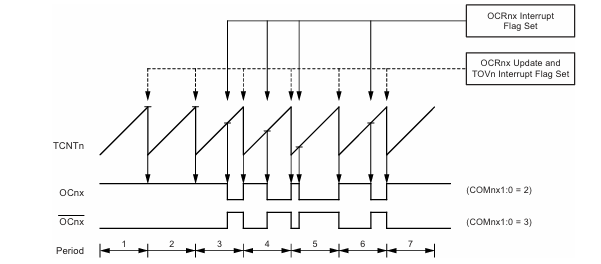
\includegraphics[width=0.35\textwidth]{anexos/Marco Teorico/Fast PMW.png}
    \caption{Diagrama de funcionamiento del modo Fast PWM en el ATmega328P. La señal de salida cambia cuando el contador alcanza el valor de comparación.}
    \label{fig:fast_pwm}
\end{figure}

\begin{figure}[H]
    \centering
    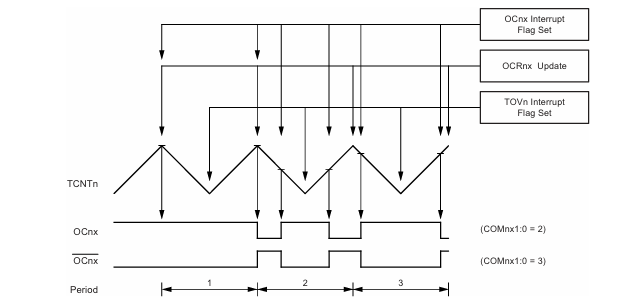
\includegraphics[width=0.35\textwidth]{anexos/Marco Teorico/Phase Correct.png}
    \caption{Modo Normal de operación del temporizador. El contador incrementa hasta su valor máximo y luego se reinicia, sin modificar las salidas.}
    \label{fig:normal_mode}
\end{figure}

\subsection{Aplicaciones}

La modulación PWM es ampliamente utilizada en sistemas embebidos, especialmente para:
\begin{itemize}
    \item Control de velocidad de motores de corriente continua.
    \item Regulación de intensidad luminosa en LEDs.
    \item Control de servomotores (por ejemplo, SG90).
    \item Conversión digital-analógica por filtrado de la señal PWM.
\end{itemize}

En este trabajo práctico, el modo \textbf{Fast PWM} del \texttt{Timer0} se empleó para controlar tanto la potencia disipada en los transistores TIP31 como la velocidad del ventilador mediante el ajuste dinámico del ciclo de trabajo.

